\chapter{Defining refactoring-oriented clone types}\label{chap:clonetypes}
In section \ref{chap:backgroundclonetypes} we introduced the four clone types as defined in literature. These simple definitions are suitable for analysis of a codebase. Their detection results in simple to understand numbers to argue about a codebase. However, these clone types have a few flaws which makes it hard to argue to what extend two fragements of code are functionally related. For each of type 1-3 clones~\cite{roy2007survey} we list our solutions to their shortcomings to increase the chance that we can merge the clone while improving the design. Due to the serious challenges involved in their detection and refactoring, type 4 clones are not considered in this study.

We also look into clone detection tools for their suitability to support the proposed clone type definitions. We selected a few criteria  Most clone detection tools support these definitions of clone types. However, many of these tools use a vastly different approach. A study by Saini et al \cite{saini2018towards} outlines different clone detection tools and compares their results for each of type 1-3 clones. Even though they operate on the same type definitions, the tools used in this study yield different results.

\section{Shortcomings of clone types}
The clone definitions, as outlined in section \ref{chap:backgroundclonetypes}, allow reasoning about the duplication in a software system. Clones by these definitions can relatively easily and efficiently be detected. This has allowed for large scale analyses of duplication. However, these clone type definitions have shortcomings which makes the clones detected in correspondance with these definitions less valuable.

In this section we discuss the shortcomings of the different clone type definitions which make them less suitable for refactoring. Because of that, these clones require more human judgement whether they should and can be refactored.

\subsection{Type 1 clones}
Type 1 clones are identical clone fragments except for variations in whitespace and comments \cite{roy2007survey}. Although textually equal, method calls can still refer to different methods, type declarations can still refer to different types and variables can be of a different type. In such cases refactoring opportunities could be invalidated.

\section{Refactoring-oriented clone types}
To resolve the shortcomings of clone types as outlined in the previous section, we propose alternative definitions for clone types to be directed at detecting clones that can and should be refactored. We have named these clones type nR clones, where n corresponds with the type definition it is modeled after. The ``R'' stands for refactoring-oriented (and may be less suitable for other analyses). Type 1R clones differ from type 1 clones as follows:

\subsection{Type 1R clones} \label{chap:type1clones}
We propose an alternative definition of type 1 clones.
\begin{itemize}
  \item \textbf{Compare the equality of the fully qualified method signature for method references.} If an identifier is fully qualified, it means we specify the full location of its declaration (e.g. \texttt{com.simonbaars.fruitgame.Apple} for an \texttt{Apple} object). This way we can validate whether two method references, like method calls, are functionally equal. In the method signature, not only the fully qualified identifier of the method should be considered, but also the type of all its arguments. This way we can be sure that two potentially cloned method references do not point to overloaded variants (in a case that the data type of arguments is overloaded).
  \item \textbf{Compare the equality of the fully qualified identifier for type references.} This way we can be sure that two referenced types are actually equal, and that they are not just two types with the same name.
  \item \textbf{Compare the equality of the fully qualified identifier for variable usages.} Two cloned lines might use a variable with the same name, but different types. This might pose serious challenges on refactoring, as the variables might not concern the same object or primitive. To check this, we need to track the declaration of variables and from this infer the fully qualified identifier of its type.
  \item \textbf{Compare the equality of the fully qualified identifier for method references and call signatures.} This is to prevent a change in functionality after merging the clone, as methods with equal names/parameters can still contain different functionality.
\end{itemize}

%% ADDED
\begin{wrapfigure}{r}{5.5cm}
\caption{A wrapped figure going nicely inside the text.}\label{wrap-fig:1}
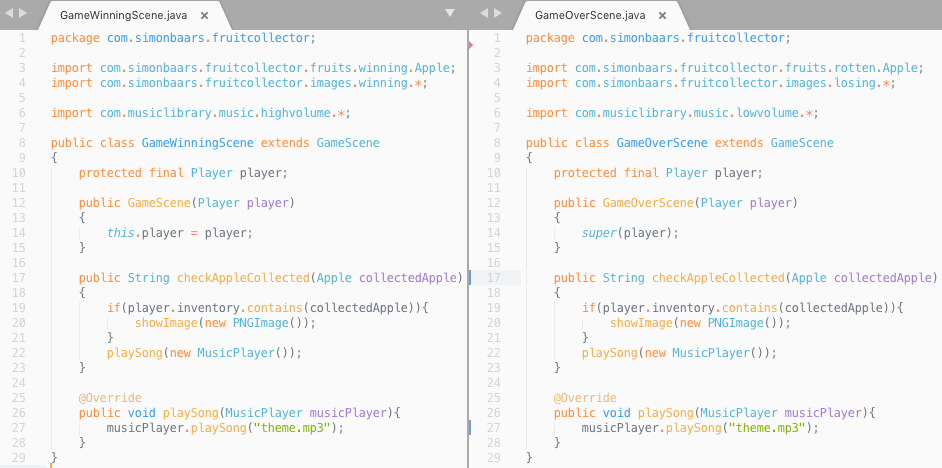
\includegraphics[width=5.5cm]{img/type-1-not-cloned}
\end{wrapfigure}
%% END ADDED

\section{Type 2R clones}
Type 2 clones allow any change in identifiers, literals, types, layout, and comments. For refactoring purposes, this definition is unsuitable; if we allow any change in identifiers, literals, and types, we cannot distinguish between different variables, different types and different method calls anymore. This could render two methods that have an entirely different functionality as clones. Merging such clones can be harmful instead of helpful.

We tackle these problems with type 2R clones to be able to detect such clones that can and should be merged. Our definition ensures functional similarity by applying the following changes to type 2 clones:

\begin{itemize}
  \item \textbf{Considering types:} Type 2 clones do not consider types. However, this can make a code fragment very hard to refactor, as different types can describe different functional concepts. Because of this, we propose that type 2R clones should consider types like type 1R clones do.
  \item \textbf{Having a distinction between different variables:} For type 2 clones, no identifiers would be taken into account. We agree that a difference in identifiers may still result in a harmful clone, but we should still consider the distinction between different variables. For instance, if we call a method like this: \texttt{myMethod(var1, var2)}, or call this method like this: \texttt{myMethod(var1, var1)}. Even if the variables have the same type, the distinction between the variables is important to ensure the functionality is the same after merging.
  \item \textbf{Defining a threshold for variability in literals:} For type 2 clones no literals would be taken into account. We agree, as when merging the clone (for example by extracting a method), we can turn the literal into a method parameter. However, we would argue that thresholds matter here. How many literals may differ for the segment still to be considered a clone with another segment? We need to define a threshold to be sure that, by merging, we are not replacing a code fragment by a worse maintainable design.
  \item \textbf{Consider method call signatures and define a threshold for variability in method calls:} As type-2 clones allow changes in identifiers, also the names of called methods may vary. However, because of this, completely different methods can be called in cloned fragments as a result. This poses serious challenges on refactoring and makes it more disputable whether such a clone is harmful for the maintainability of the code. This is because different method identifiers can describe a completely different functionality. Therefore, we suggest considering the call signatures of cloned methods when they are compared. We can allow variability in the rest of method identifiers by passing the function as a parameter. To limit the amount of parameters required we also recommend defining a threshold for variability in method call expressions, so only a limited number of method calls can vary.
\end{itemize}

\section{Type 3R clones}
Type 3 clones are even more permissive than type 2 clones, allowing added and removed statements. For these clones, thresholds matter a lot to make sure that not the whole project is detected as a clone of itself. The main question for this study regarding type 3 clones is: \textit{``how can we merge type 3 clones while improving the design?''}.

Clone instances in type 3 clones are almost always different in functionality. As we have to ensure equal functionality after merging the clone, we have to wrap the difference in statements between the clone instances in conditional blocks. We can then pass a variable to indicate which path should be taken through the code (either a boolean or an enumeration). Such a refactoring would make added statements that are contiguous less harmful for the design than added statements that are scattered throughout the cloned fragment.

We also argue that statements that are not common between two clone instances, should not count towards the size of the clone (and thus towards the threshold which determines whether the clone will be taken into account). As for the detection of type 3 clones, we think the easiest opportunity to detect these clones is to consider it as a postprocessing step after clone detection. By trying to find short gaps between clones, we can find opportunities to merge clone classes into a single type 3 clone class. The amount of statements that this ``short gap'' can maximally span should be dependent on a threshold value.

\section{The challenge of detecting these clones}\label{chap:challenge}
To detect each type of clone, we need to parse the fully qualified identifier of all types, method calls and variables. This comes with serious challenges, regarding both performance and implementation. Also, to be able to parse all fully qualified identifiers, and trace the declarations of variables, we might need to follow cross file references. The referenced types/variables/methods might even not be part of the project, but rather of an external library or the standard libraries of the programming language. All these factors need to be considered for the referenced entity to be found, on basis of which a fully qualified identifier can be created.

CloneRefactor uses JavaParser \cite{tomassetti2017javaparser}. JavaParser has a built-in symbol solver, which can automatically resolve types, method calls and variables. However, because of this, CloneRefactor does require all libraries that the software project requires (apart from the Java Standard Library). If these are not available, CloneRefactor will estimate types on basis of the information that is available.

\section{Suitability of existing Clone Detection Tools towards our refactoring purposes}
\label{ch:tool-overview}
We conducted a short survey on (recent) clone detection tools that we could use to analyze refactoring possibilities. The results of our survey are displayed in table~\ref{table:dettools}. We chose a set of tools that are open source and can analyze a popular object-oriented programming language. Next, we formulate the following four criteria by which we analyze these tools:
\begin{enumerate}
    \item \textbf{Should find clones in any context.} Some tools only find clones in specific contexts, such as only method-level clones. We want to perform an analysis on all clones in projects to get a complete overview.
\item \textbf{Should find all clones in created control projects.} We assembled a number of test projects to assess the validity of clone detection tools. On basis of this, we checked whether clone detection tools can correctly find clones in diverse contexts.
\item \textbf{Can analyse resolved symbols.} When detecting clones for refactoring purposes, it is important that clone instances can be merged. Sometimes, textual equality between code fragments does not imply that these can be merged (this is described more elaborately in section \ref{chap:type1clones}). Because of this, we want to use a clone detection tool that can analyze such structures.
\item \textbf{Extensive detection configuration.} We aim to exclude expressions/statements from matching (more about our rationale in section~\ref{chap:clonetypes}). To achieve this, the tool needs to be able to allow those threshold changes. This can be either through simple changes of the source code, or by using some configuration file.
\end{enumerate}

\begin{table}[H]
 \begin{center}
  \caption{Our survey on clone detection tools.} \label{table:dettools}
  \medskip
\begin{tabular}{|l|l|l|l|l|l|}
\hline
\textbf{Clone Detection Tool} & \textbf{(1)} & \textbf{(2)} & \textbf{(3)} & \textbf{(4)} \\ \hline
Siamese \cite{ragkhitwetsagul2019siamese} &  &             &             & \checkmark            \\ \hline
NiCAD \cite{roy2008nicad, cordy2011nicad} & \checkmark                             & \checkmark            &             &             \\ \hline
CPD \cite{roy2009comparison} & \checkmark & \checkmark            &             &             \\ \hline
\begin{tabular}[c]{@{}l@{}}CCFinder \cite{kamiya2002ccfinder}\\ D-CCFinder \cite{livieri2007very}\end{tabular} & \checkmark  & \checkmark   &    &   \\ \hline
CCFinderSW \cite{semura2017ccfindersw}   & \checkmark     &             &             & \checkmark            \\ \hline
\begin{tabular}[c]{@{}l@{}}SourcererCC \cite{sajnani2016sourcerercc}\\ Oreo \cite{saini2018oreo}\end{tabular} & \checkmark    &             &             & \checkmark            \\ \hline
BigCloneEval \cite{svajlenko2016bigcloneeval}  & \checkmark  & \checkmark   &             &             \\ \hline
Deckard \cite{jiang2007deckard} & \checkmark   &             & \checkmark            &             \\ \hline
Scorpio \cite{higo2013revisiting, kamalpriya2017enhancing} & \checkmark   &     & \checkmark  & \checkmark   \\ \hline
\end{tabular}
\end{center}
\end{table}

None of the state-of-the-art tools we identified implement all our criteria, so we decided to implement our own clone detection tool: CloneRefactor\footnote{CloneRefactor (WIP) is available on GitHub: \url{https://github.com/SimonBaars/CloneRefactor}. This repository contains all scripts that were used to retrieve the data that is displayed in this paper.}.

\chapter{Evaluation setup}
In this chapter we describe the setup we use for our experiments. Our most prominent contribution is the proposal of a tool called CloneRefactor. This tool allows us to map clones with all clone definitions as described in chapter \ref{chap:clonetypes}.

All data for our experiments, as displayed in chapter \ref{ch:results}, is measured over a corpus of Java projects. In this chapter we will explain how we prepared this corpus.

\section{CloneRefactor}
CloneRefactor is the name of our clone detection and refactoring tool. It features the following novel functions:
\begin{itemize}
  \item Detection of clone classes rather than clone pairs.
  \item A novel detection method, aimed at extensibility.
  \item Detection of refactoring-oriented clone types, in addition to the literature clone types.
  \item Allows for automated refactoring of a subset of the detected duplication issues.
\end{itemize}
In this section we describe our approach and rationale for the design decisions regarding this tool.

\subsection{JavaParser}
A very important design decision for CloneRefactor is the usage of a library named JavaParser \cite{tomassetti2017javaparser}. JavaParser is a Java library which allows to parse Java source files to an abstract syntax tree (AST). JavaParser allows to modify this AST and write the result back to Java source code. This allows us to apply refactorings to the detected problems in the source code.

Integrated in JavaParser is a library named SymbolSolver. This library allows for the resolution of symbols using JavaParser. For instance, we can use it to trace references (methods, variables, types, etc) to their declarations (these referenced identifiers are also called `symbols`). This is very useful for the detection of our refactoring-oriented clone types, as they make use of the fully qualified identifiers of symbols.

In order to be able to trace referenced identifiers SymbolSolver requires access to not only the analyzed Java projects, but also all its dependencies. This requires us to include all dependencies with the project. Along with this, SymbolSolver solves symbols in the JRE System Library (the standard libraries coming with every installation of Java) using the active Java Virtual Machine (JVM). This has a big impact on performance efficiency.

Because of the requirement of symbol resolution, the refactoring-oriented clone types are less suitable for large scale clone analysis.

\subsection{Clone Detection}
To detect clones, CloneRefactor parses the AST aqcuired from JavaParser to an unweighted graph structure. This graph structure is then

\section{The corpus}\label{chap:corpus}
For our measurements we use a large corpus of open source projects \cite{githubCorpus2013}. This corpus has been assembled to contain relatively higher quality projects. Also, any duplicate projects were removed from this corpus. This results in a variety of Java projects that reflect the quality of average open source Java systems and are useful to perform measurements on.

As indicated in chapter \ref{chap:challenge} CloneRefactor requires all libraries of software projects we test. As these are not included in the used corpus \cite{githubCorpus2013}, we decided to filter the corpus to only include Maven projects. Maven is a build automation tool used primarily for Java, and works on basis of an \texttt{pom.xml} file to describe the projects' dependencies. As no \texttt{pom.xml} files are included in the corpus, we cloned the latest version of each project in the corpus. We then removed each project that has no \texttt{pom.xml} file. As a final step, we collected all dependencies for each project by using the \texttt{mvn dependency:copy-dependencies -DoutputDirectory=lib} Maven command, and removed each project for which not all dependencies were available (due to non-Maven dependencies being used or unsatisfiable dependencies being referenced in the \texttt{pom.xml} file).

Some general data regarding this corpus is displayed in Table \ref{table:general}.

\begin{table}[H]
  \begin{center}
  \caption{General results for GitHub Java projects corpus \cite{githubCorpus2013}.} \label{table:general}
  \medskip
\begin{tabular}{|l|l|}
\hline
Amount of projects                                                                                      & 1,361      \\ \hline
\begin{tabular}[c]{@{}l@{}}Amount of lines (excluding\\whitespace, comments and newlines.)\end{tabular} & 1,414,996  \\ \hline
Amount of statements/declarations                                                                       & 1,212,189  \\ \hline
\begin{tabular}[c]{@{}l@{}}Amount of tokens (excluding\\whitespace, comments and newlines.)\end{tabular} & 11,643,194 \\ \hline
\end{tabular}
\end{center}
\end{table}
